Based on the presented idea, we design and present the prototype which consists of three components (see Figure \ref{fig:figure1}):
\begin{itemize}
\item The server centrally manages all users information, bookings and machines status.
\item Each washing machine has a monitoring device which displays current states of the machine and communicate with server.
\item {\toolname} is the laundry booking application on mobile phone.
\end{itemize}
\begin{figure}[h]
\centering
  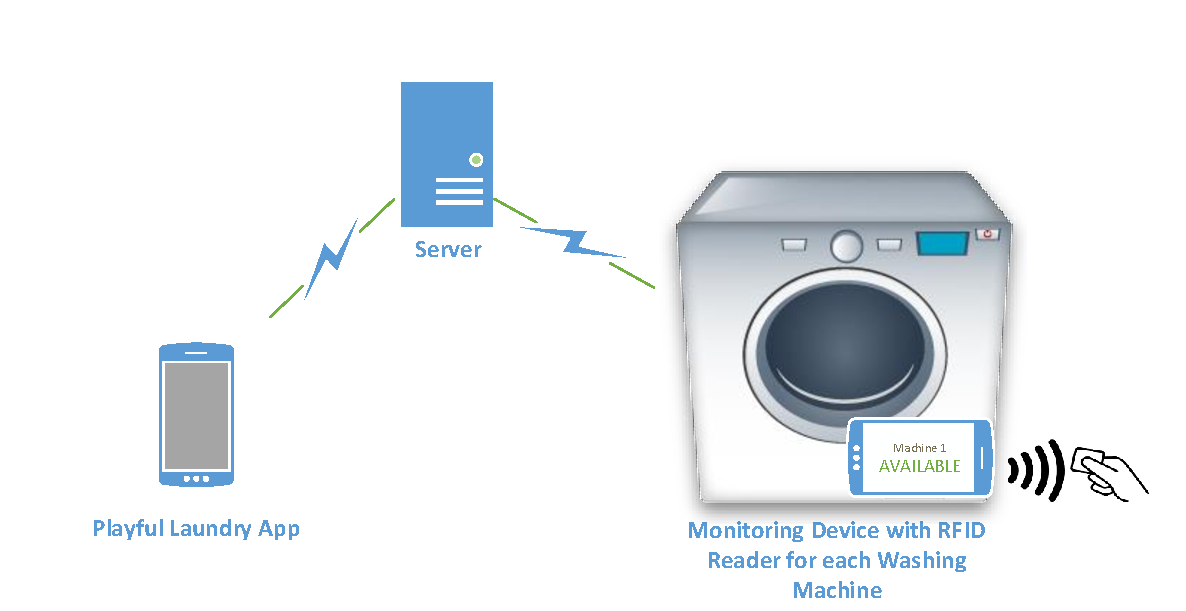
\includegraphics[width=\columnwidth]{figures/overview}
  \caption{Three components of the booking system.}~\label{fig:figure1}
\end{figure}
\subsubsection{Monitoring Device}
Each monitoring device has a RFID reader and a screen which displays interactive instructions and information of the machine such as: machine id, remaining time of current job, current state of washing machine (\emph{AVAILABE} - there is still enough time before the next reservation begins, \emph{USED IN A MOMENT} - next reservation will begin shortly, \emph{RESERVED} - the machine was already booked at that moment, \emph{IN USE} - machine is running, \emph{FINISHED} - washing has just finished), etc.
 For prototyping monitoring device, we use an android phone as a display and an arduino uno board with RFID shield (see Figure \ref{fig:figure2}).
\begin{figure}[h]
\centering
  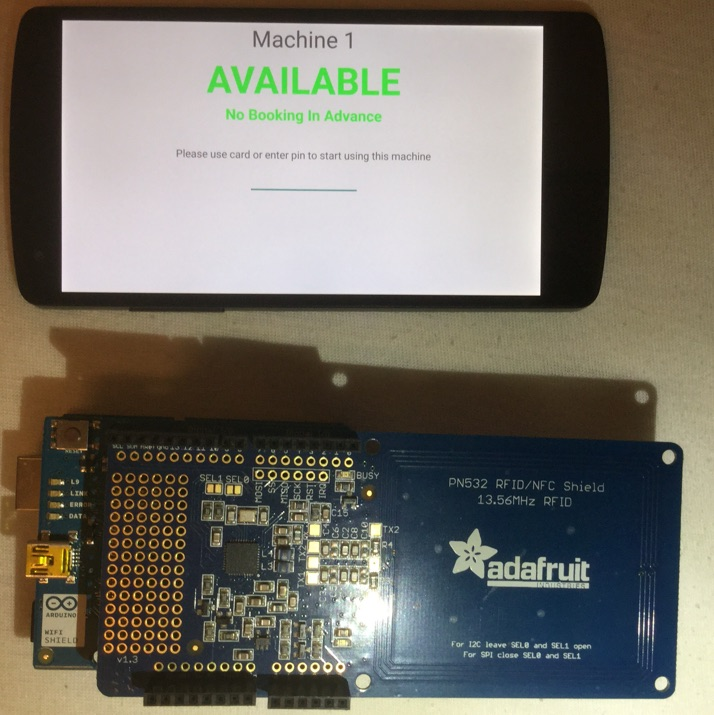
\includegraphics[width=0.7\columnwidth]{figures/Monitoring}
  \caption{The prototype of monitoring device.}~\label{fig:figure2}
\end{figure}
To activate a machine, users could either scan their RFID cards or enter PIN number. If the users already reserved the current time-slot, monitoring device would instruct them to start the machine; otherwise they have to go through booking process right on the monitoring device before using the machine.

When the machine is \emph{IN USE} or \emph{FINISHED} state, the \emph{booking id} of current session would be shown on the screen. Figure \ref{fig:figure3} shows the screenshot of the display when the machine is \emph{IN USE}. This id disappears once the users take their clothes out of the machine. Therefore, if the users are being late, other users could use this \emph{booking id} and the \emph{machine id} for reporting.
\begin{figure}[h]
\centering
  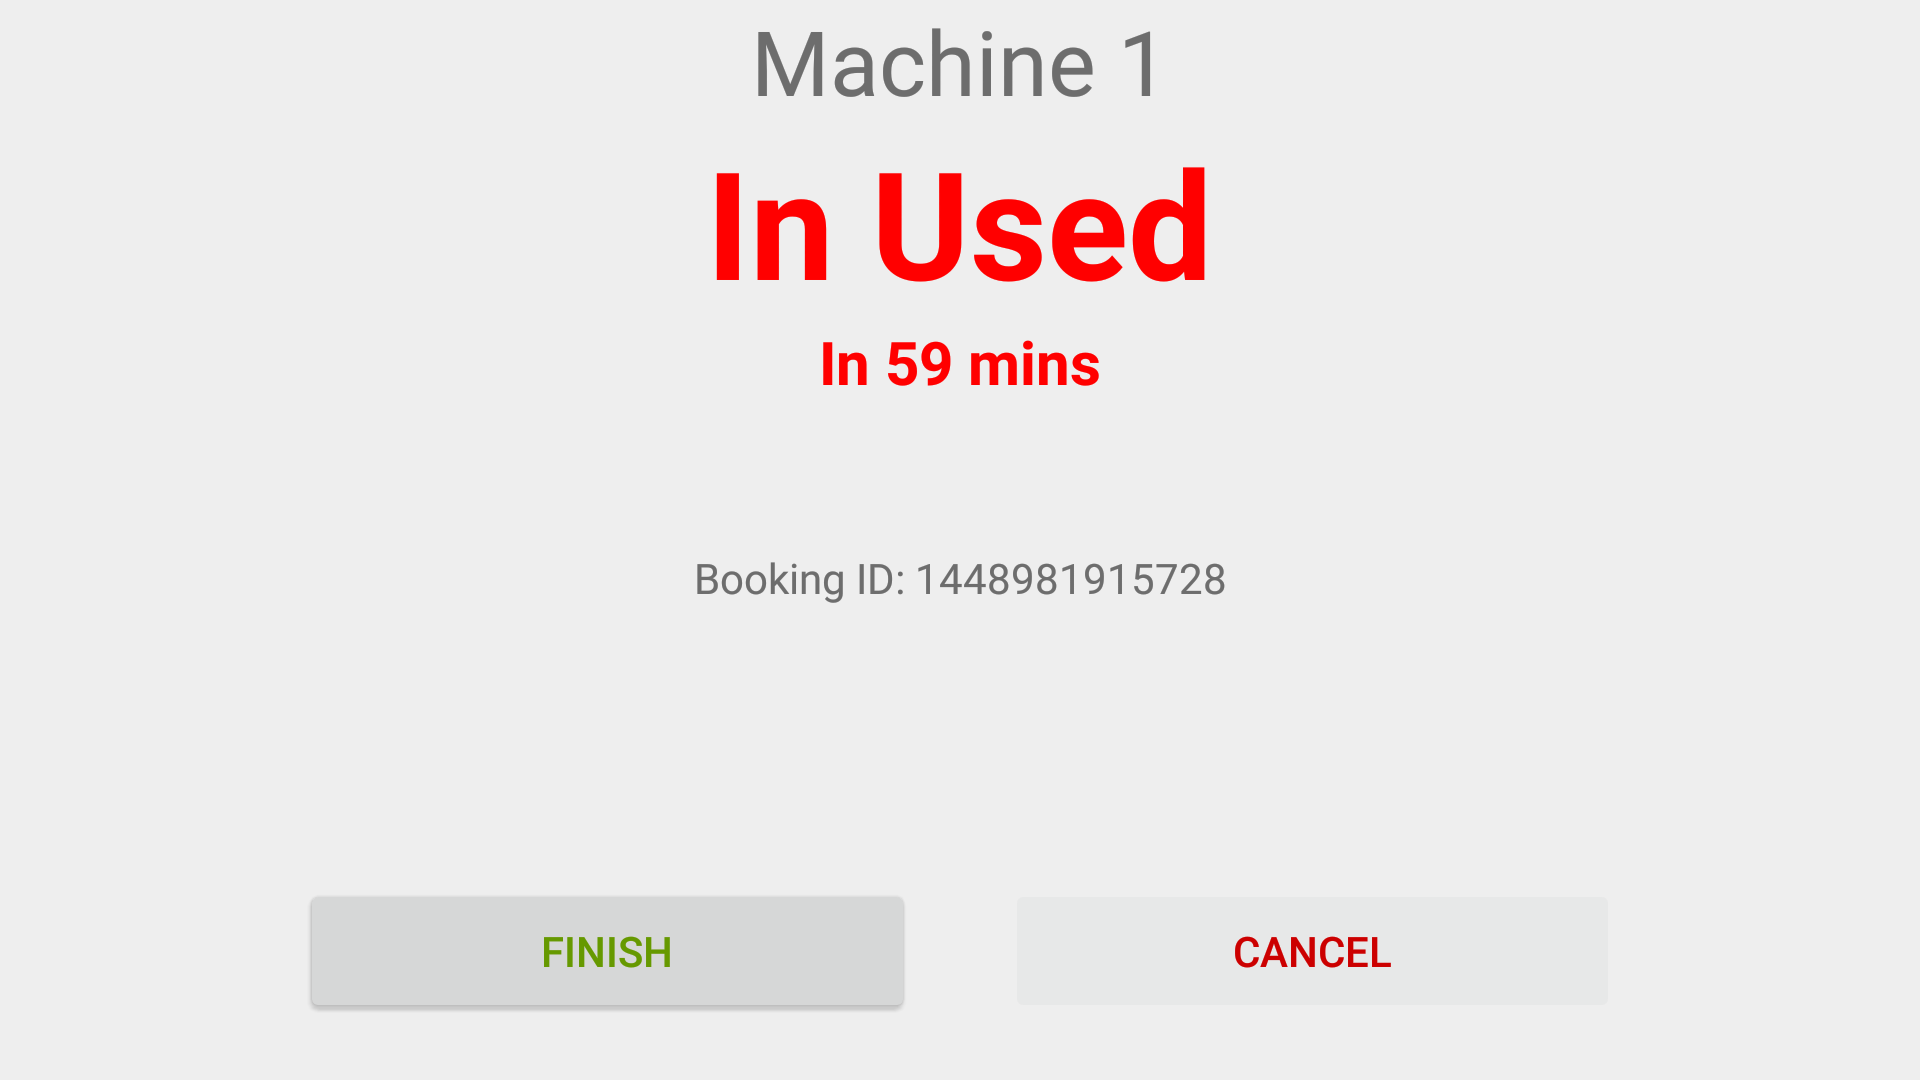
\includegraphics[width=0.8\columnwidth]{figures/inuse}
  \caption{Monitoring display when the machine is running.}~\label{fig:figure3}
\end{figure}
\subsubsection{{\toolname} Application}
{\toolname} is an Android application which allows users to reserve a washing machine, manage booking, observe the current states of the machines, etc. Figure \ref{fig:menu} shows the menu of the application.

The \emph{Booking} tab (see Figure \ref{fig:booking}) allows users to make a reservation for a specific time-slot. There is limitation on the number of time-slots user could book in a week. This number would increase when user get to higher level. Figure \ref{fig:hours} shows the booking interface with time-slots. Users would be awarded points for each time-slot they reserve. The amounts of awards depend on how popular that time-slot is.
\begin{figure*}%
    \centering
    \subfloat[Main menu]{{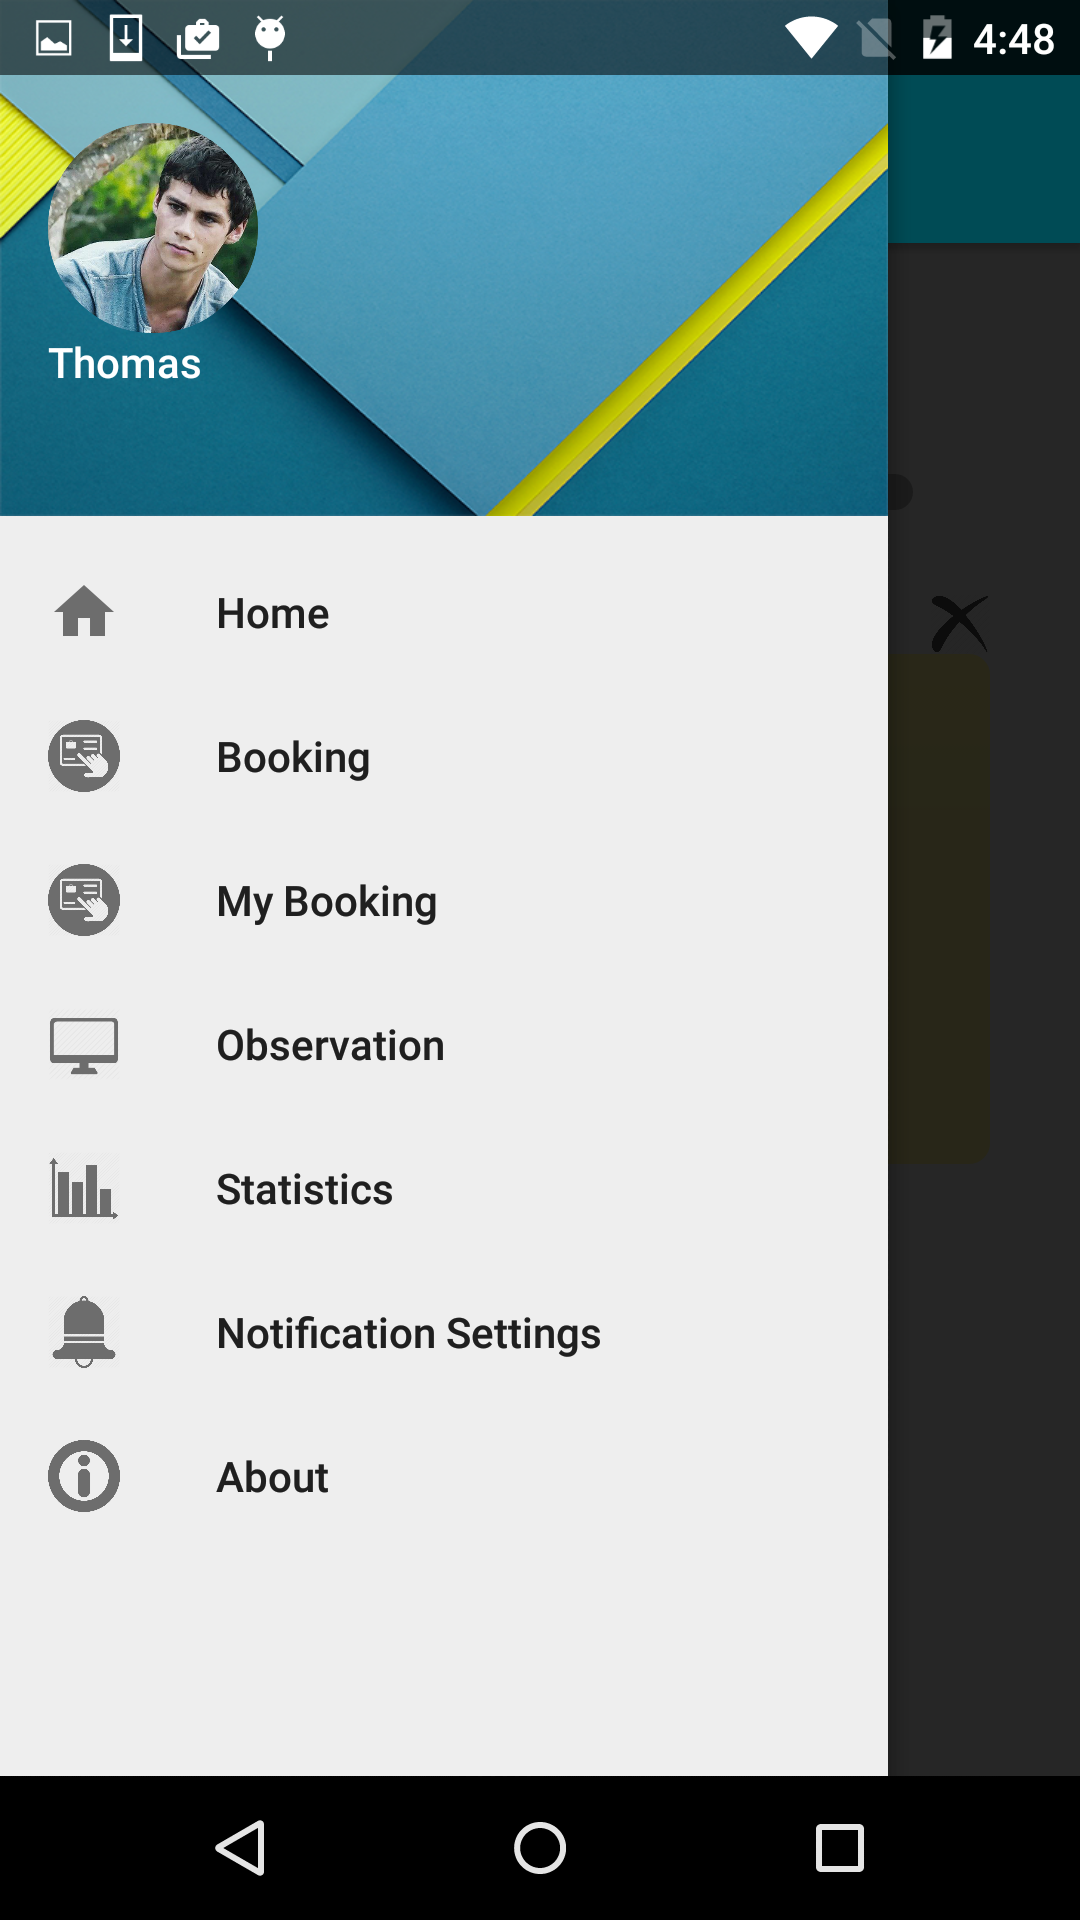
\includegraphics[width=0.4\columnwidth]{figures/menu} \label{fig:menu}}}
    %\qquad
    \subfloat[Home]{{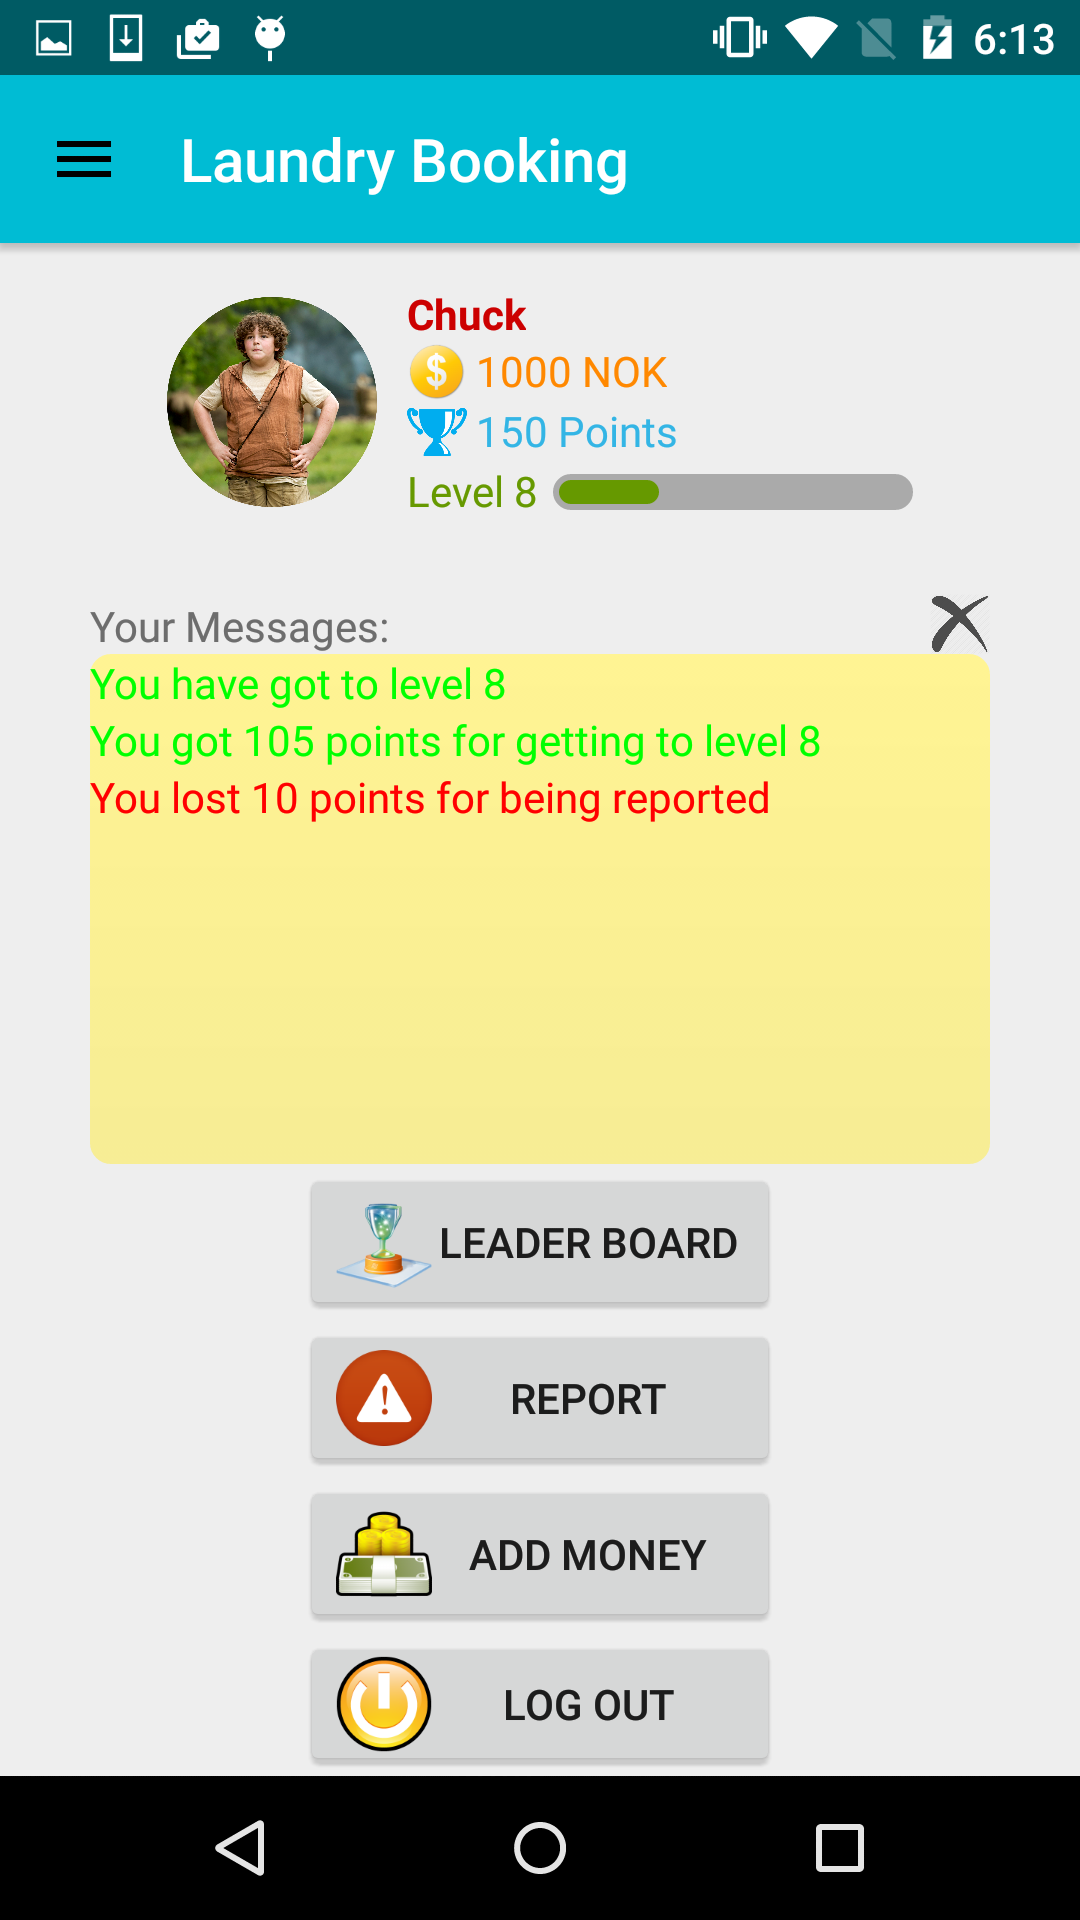
\includegraphics[width=0.4\columnwidth]{figures/home} \label{fig:home} }}
		\subfloat[Booking]{{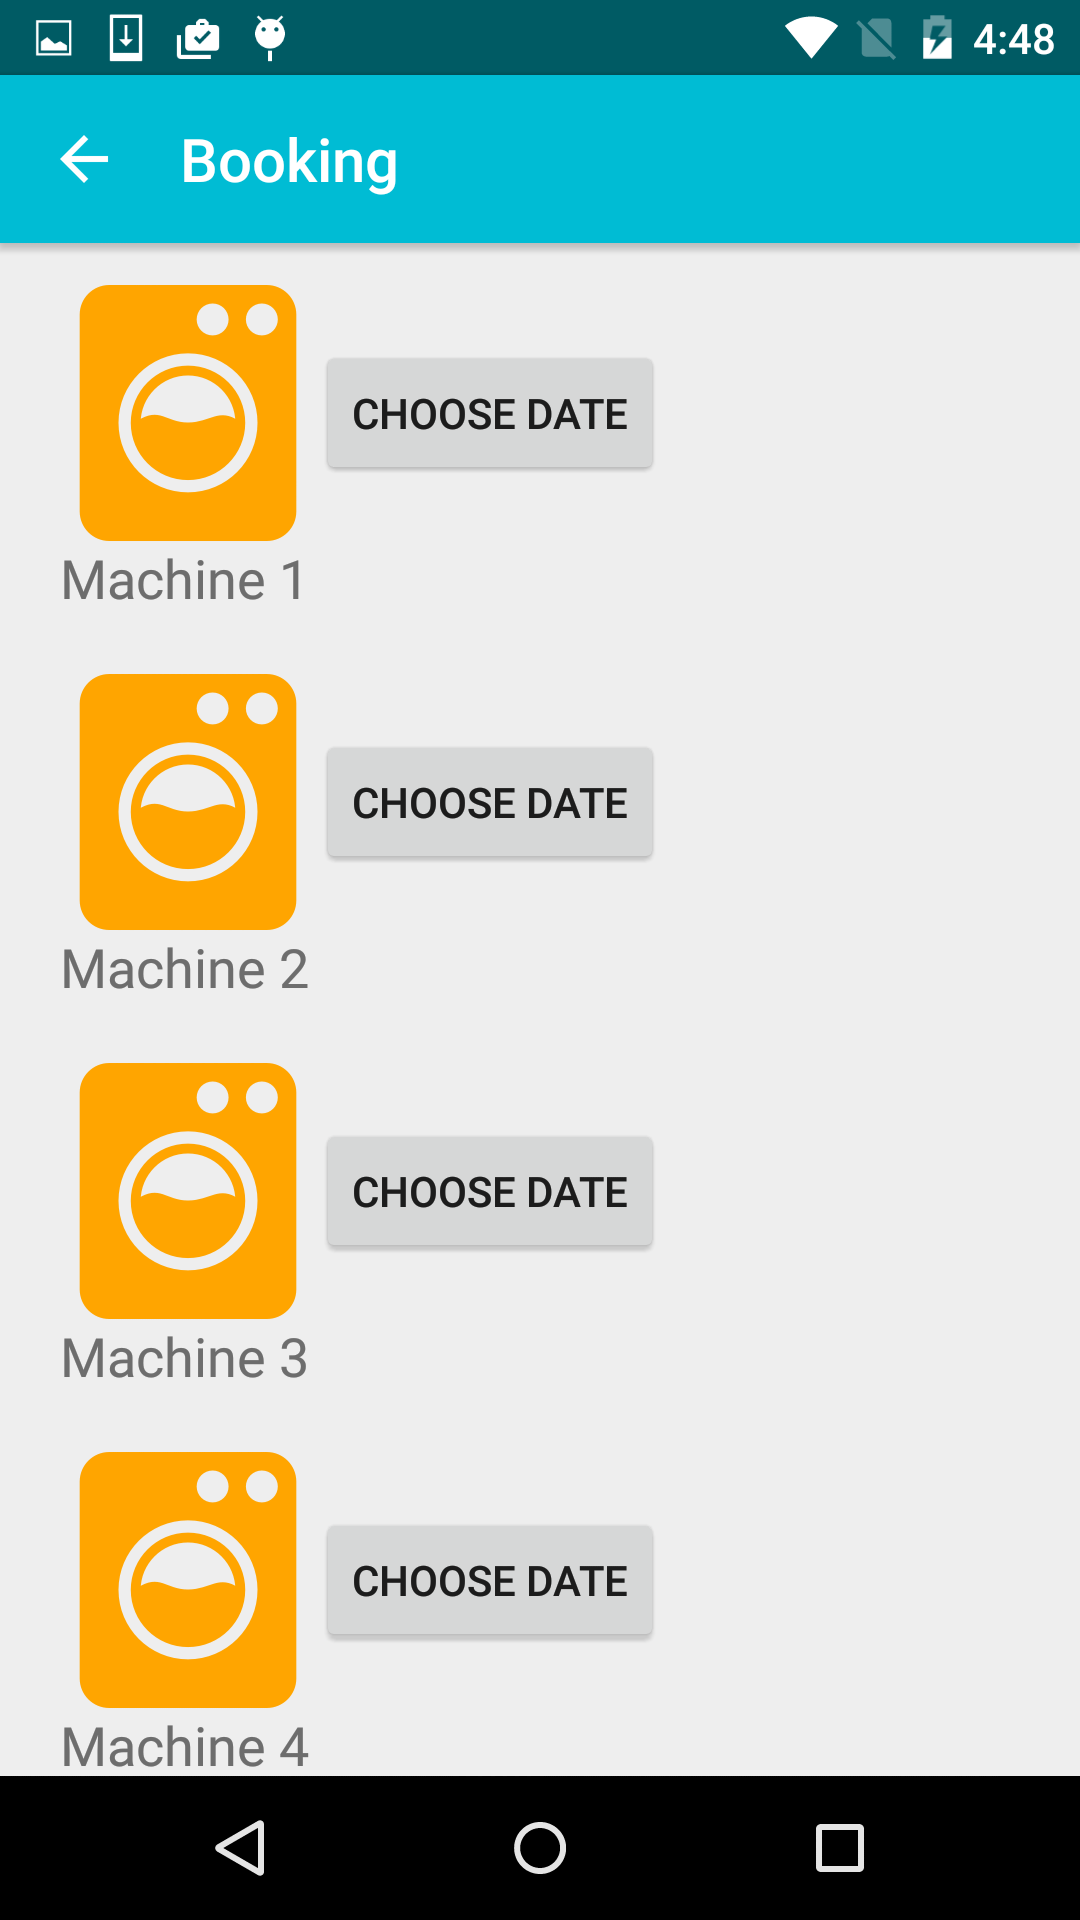
\includegraphics[width=0.4\columnwidth]{figures/booking} \label{fig:booking} }}
		\subfloat[Observation]{{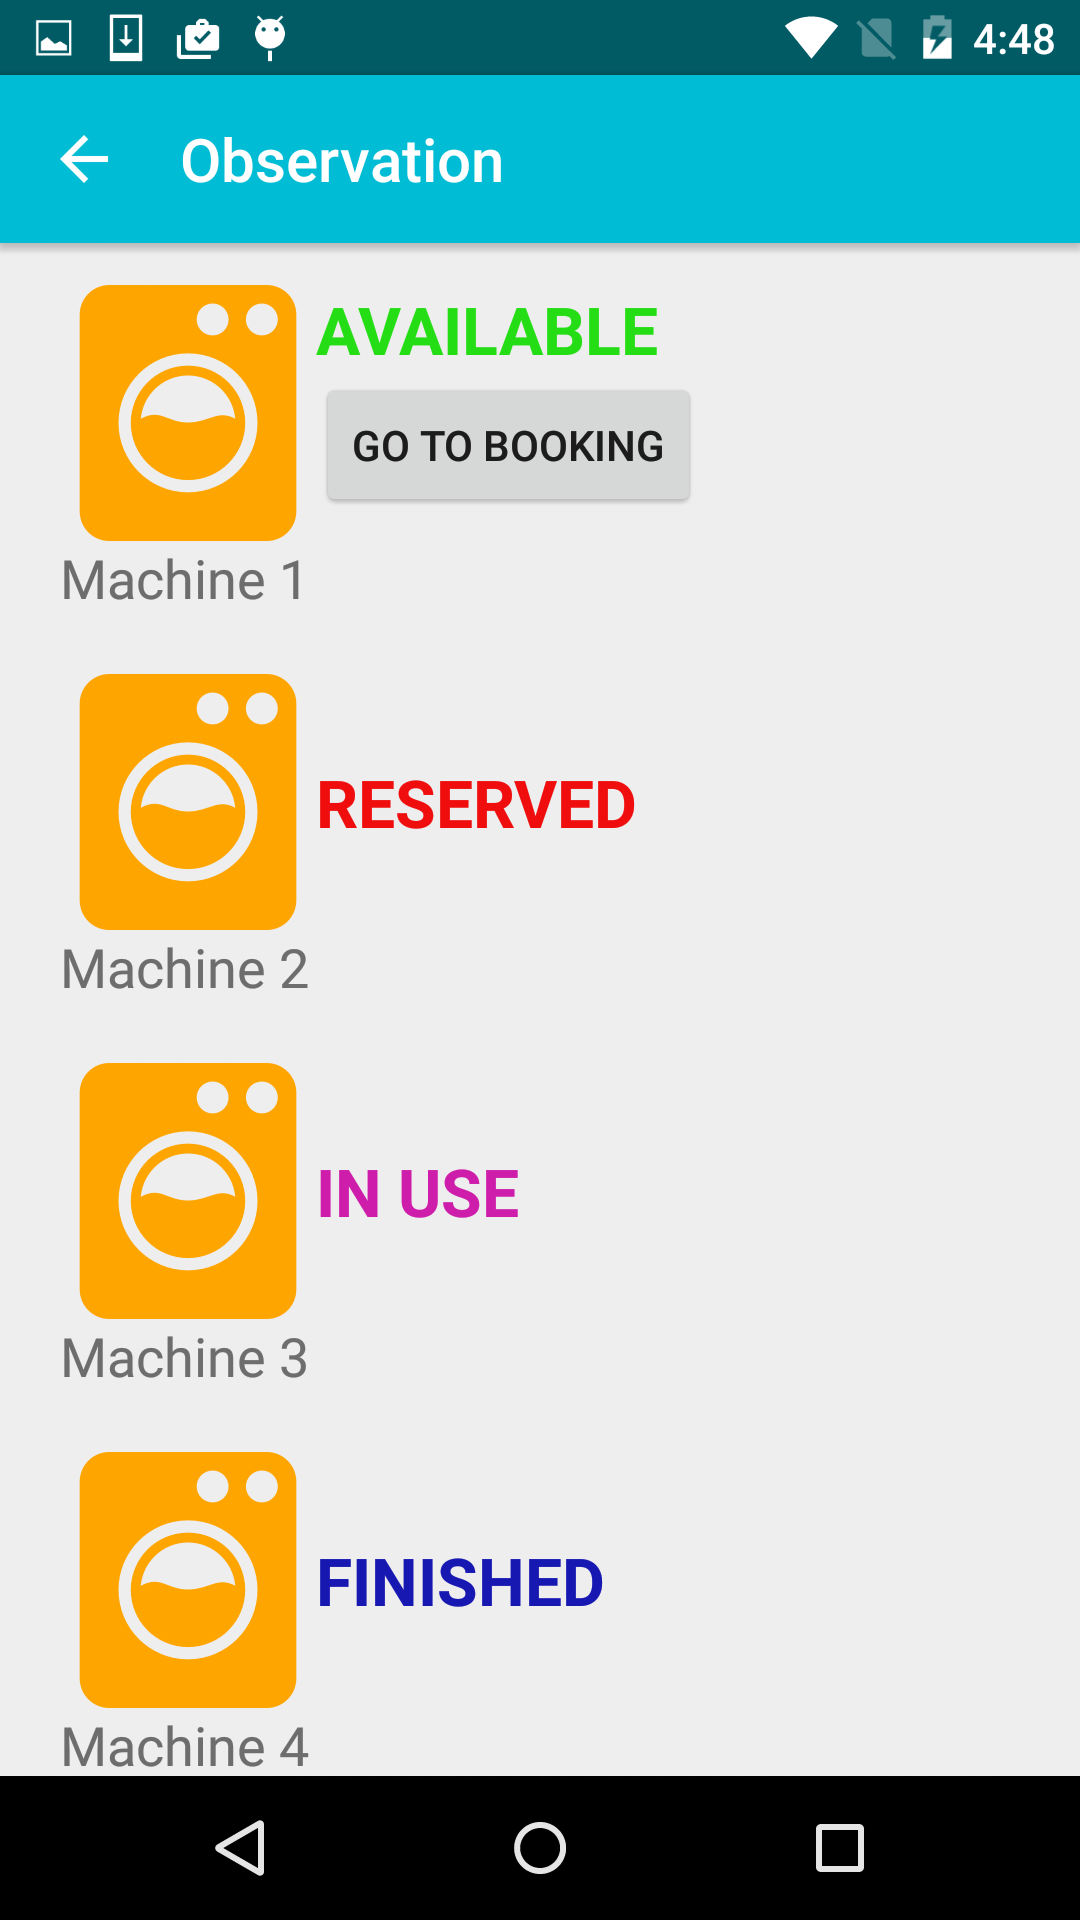
\includegraphics[width=0.4\columnwidth]{figures/observation} \label{fig:observation} }}
		\subfloat[Statistics]{{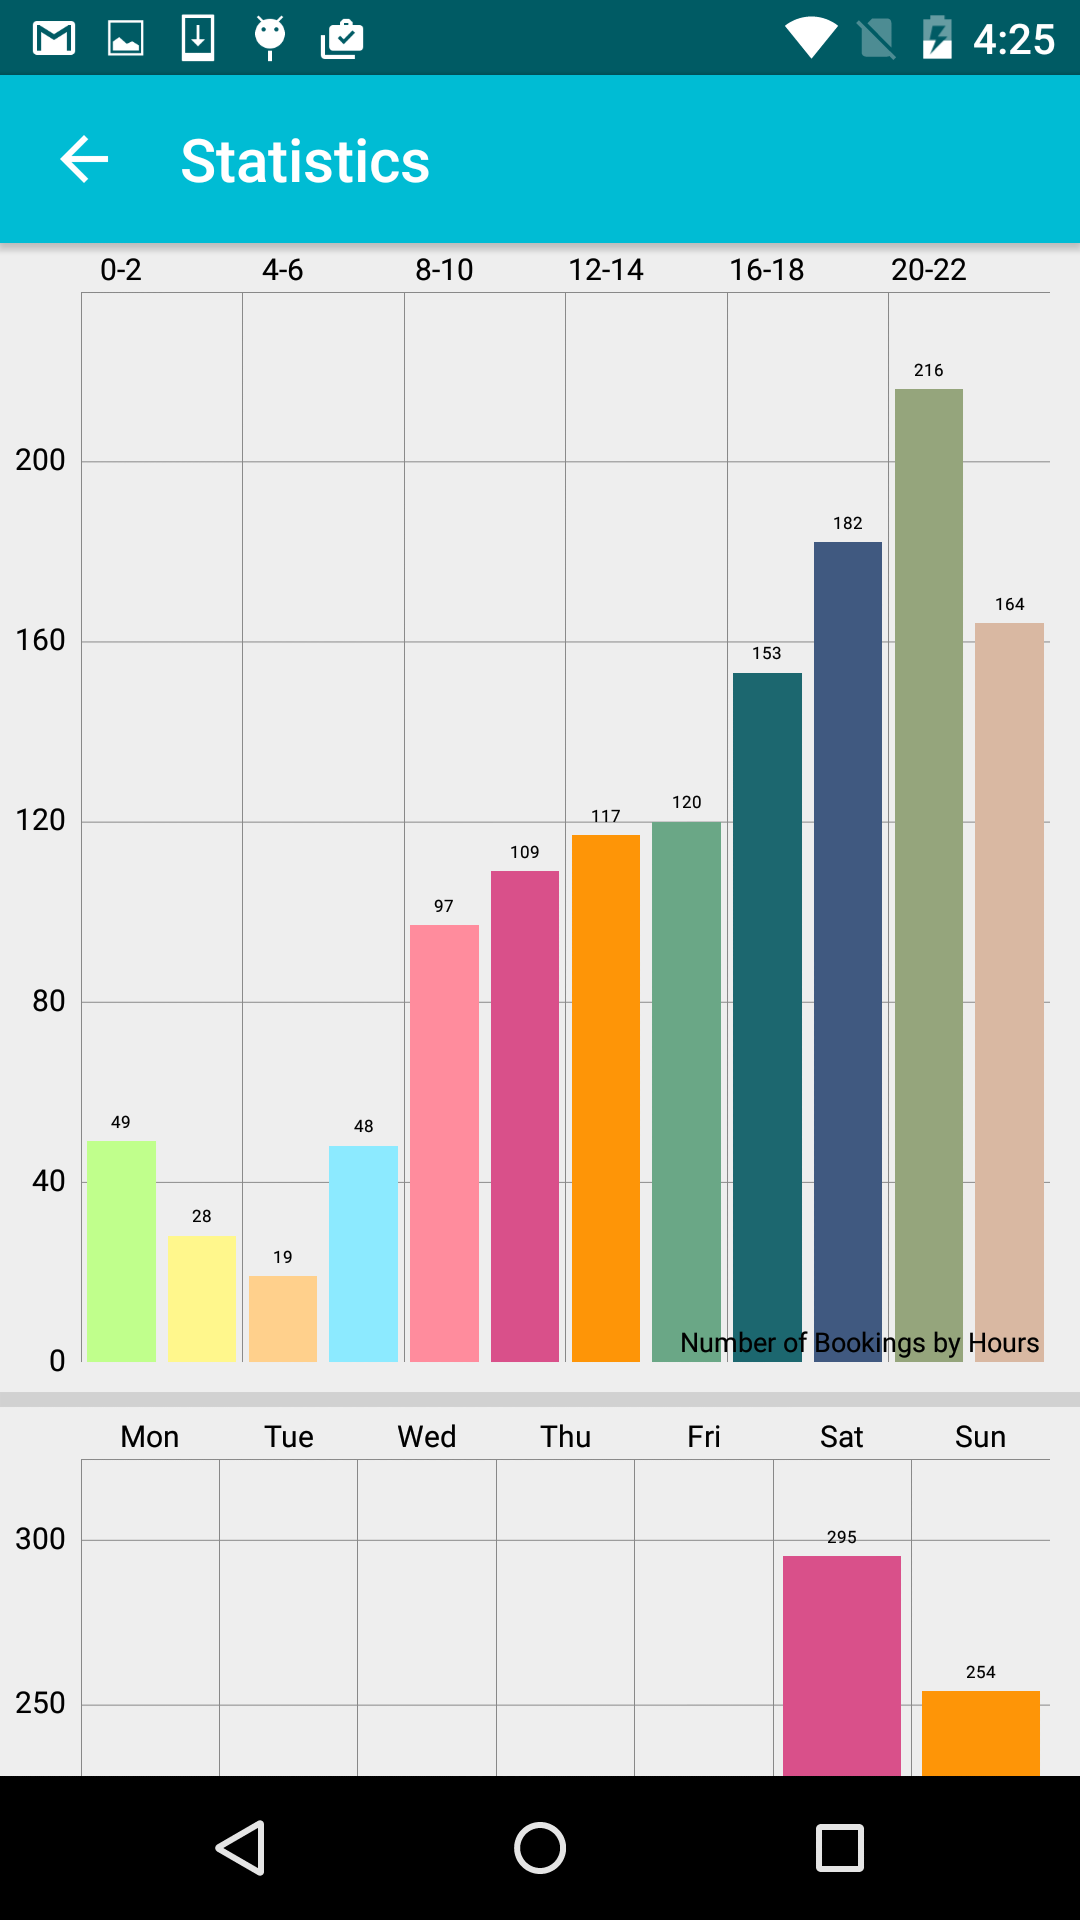
\includegraphics[width=0.4\columnwidth]{figures/stat} \label{fig:stat} }}
    \caption{User interface of \toolname.}%
    \label{fig:figure4}
\end{figure*}

In \emph{My Booking} tab, users could find all their upcoming bookings. They could also cancel a booking in this tab.

 \emph{Observation} (see Figure \ref{fig:observation}) shows the current states of all washing machine. Users could use this function to check for available machines at that moment and use it right away without booking in advance.

There are two bar charts displayed in \emph{Statistics} tab (see Figure \ref{fig:stat}). The first one illustrates numbers of bookings in previous week by hours while the second one represents these numbers by days. Users could use these statistics to plan their ``laundry strategy'' of the week.

\emph{Notification} allows users to set reminders. The application always use in-app notification to remind users for upcoming bookings or finished jobs. In addition, they could choose to set reminder by email or SMS message.
\begin{figure}[h]%
    \centering
    \subfloat[Time-slots and award points]{{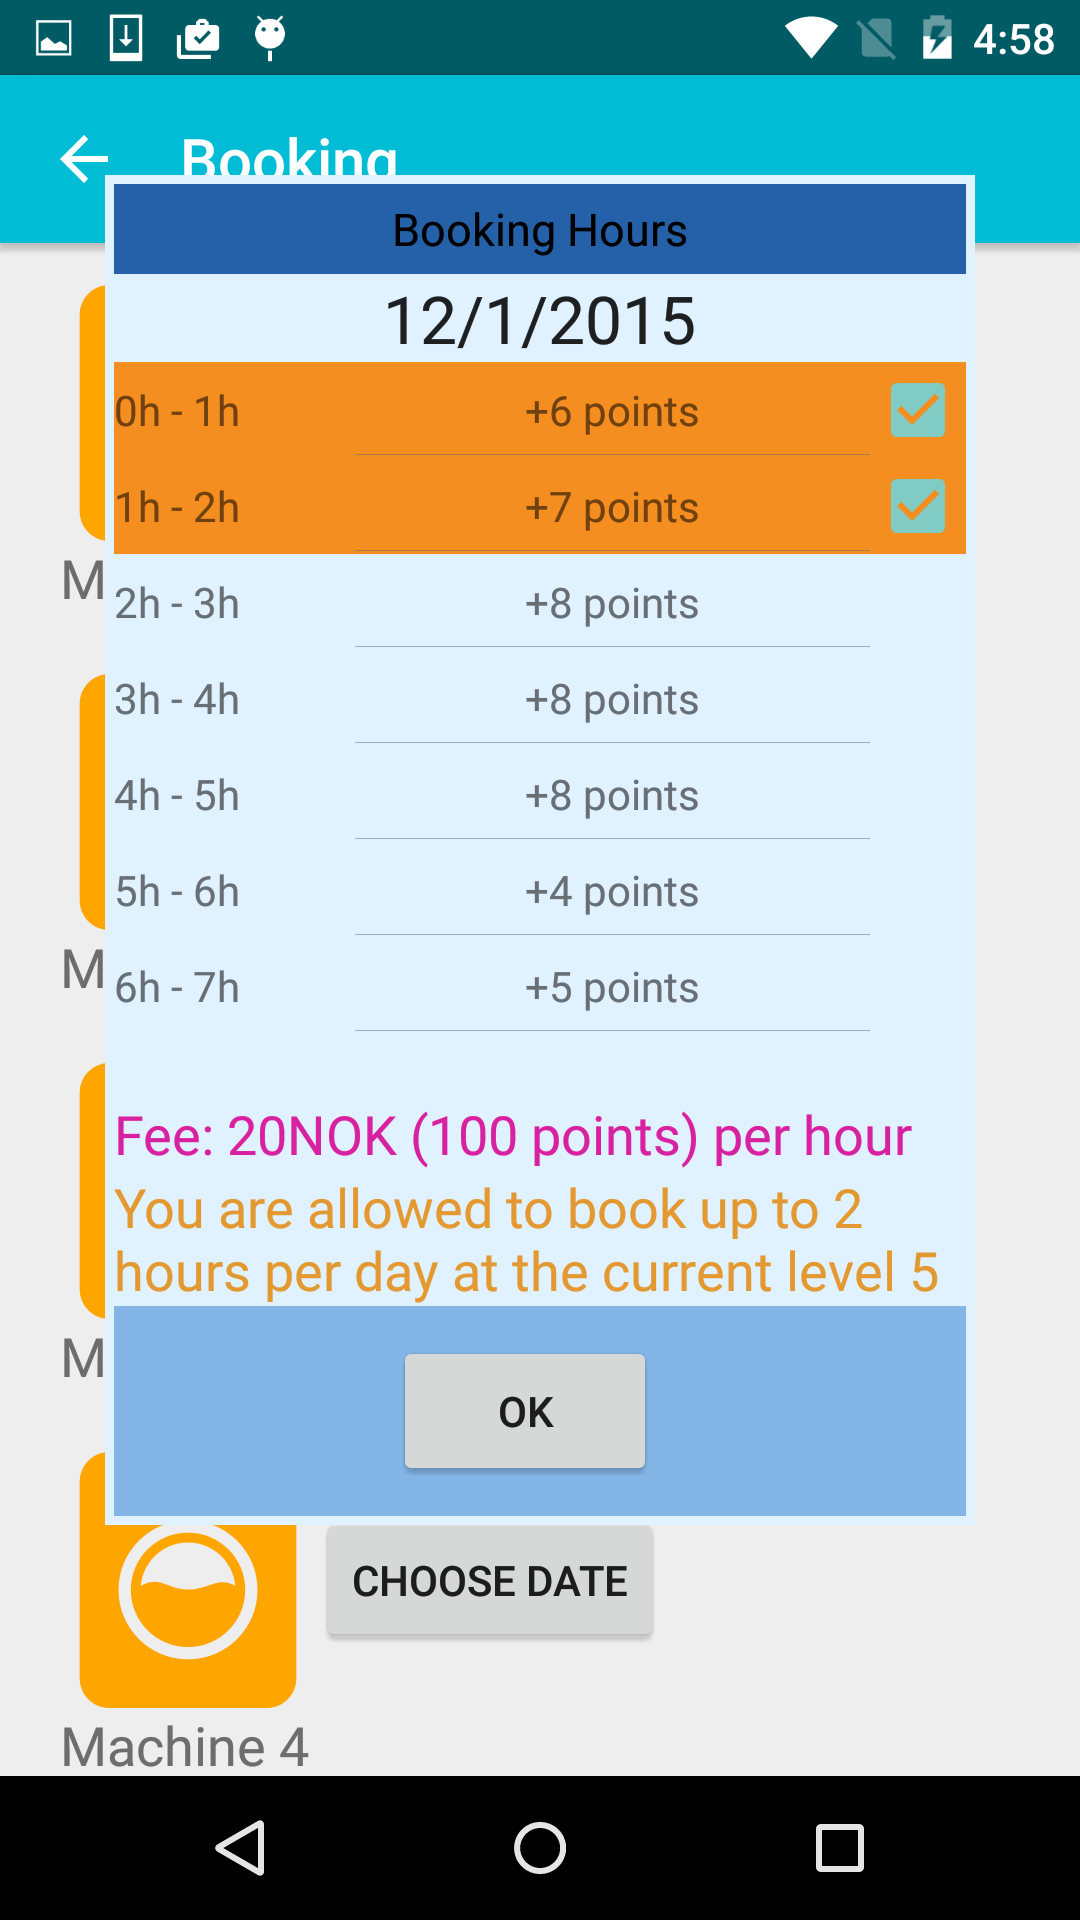
\includegraphics[width=0.4\columnwidth]{figures/hours} \label{fig:hours}}}
    %\qquad
    \subfloat[Leader Board]{{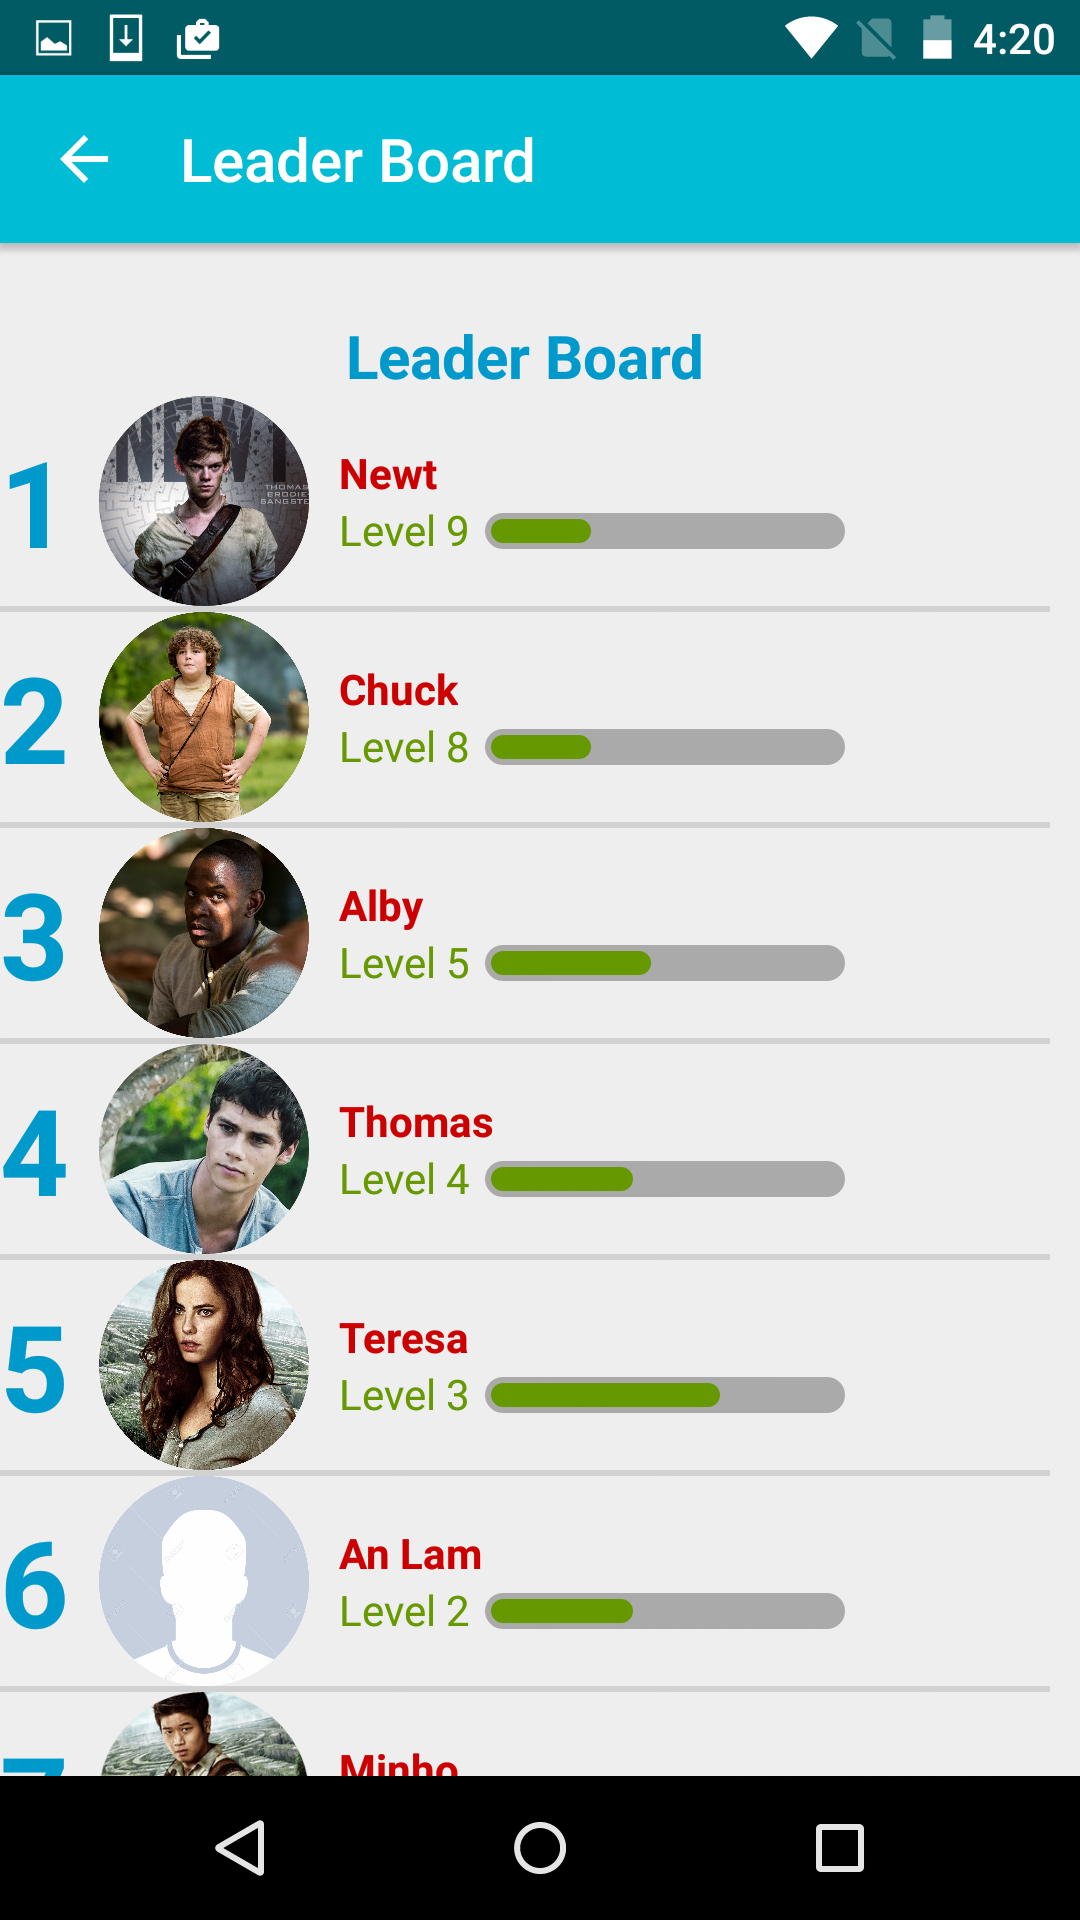
\includegraphics[width=0.4\columnwidth]{figures/leaderboard} \label{fig:leaderboard} }}
		\caption{Time-slots and Leader board.}%
    \label{fig:figure5}
\end{figure}

The \emph{Home} interface (see Figure \ref {fig:home}) displays all information about the user. This is where gamification idea is implemented. In this tab, users could find their avatars, names,  balance and points, levels and progression as well as messages about their activities. There are also buttons allowing them to access leader board (see Figure \ref{fig:leaderboard}), report a person or add money to their accounts. 